\chapter{結論}
\label{conclusion}

本章では,本研究のまとめと今後の課題を示す.

\section{本研究のまとめ}
本研究では,IPv6シングルスタックネットワークにおけるIPv4サービス提供手法として,ステートレスアドレス変換を利用した"SIIT-DC"と呼ばれるネットワークデザインに注目し,冗長性や変更追従性の問題を解決するために,考えられるアプローチを比較した上で,動的経路制御プロトコルであるBGPを利用したアドレス変換テーブルの広告・制御プロトコルを設計した.

本手法を評価するために,OSS及び自作のを利用したPoCを実装し,30台のBR,2台のルートリフレクタ,最大600台のサーバからなる評価用ネットワークにて2つのシナリオからなる評価実験を行った.
本評価実験の結果,本手法がSIIT-DCの冗長性と変更追従性を改善するフィジビリティを十分に有することが明らかになった.

\section{よりスケーラブルなBGPコネクショントポロジについての検討}
\label{conclusion:tree}
本評価実験を通して,ルートリフレクタが保有するべきBGPコネクションの数が大きくなることが,IPv4サービス提供サーバの収容可能台数と変更追従性に影響を及ぼすことがわかっている.

これはBGPコネクショントポロジを階層的なものにすることで,よりスケーラブルに本提案手法を運用することが可能である.
本節では2層のツリー型トポロジで接続されたルートリフレクタ群のスケーラビリティを定式化し,本提案手法の潜在的なスケーラビリティを明らかにする.

\subsection{2層のツリー型コネクショントポロジ}
\label{conclusion:tree:2layer}

ルートリフレクタが収容可能なサーバ台数を拡大するBGPコネクション設計に,ツリー型トポロジによるルートリフレクタの多層化の活用を考案した.
本研究において,ルートリフレクタの多層化とは,ルートリフレクタ間でツリートポロジ型のコネクションを確立させるようにルートリフレクタを配置する手法と定義する.

2層のツリー型トポロジで接続されたSIIT-DCの各ノードの関係図\ref{fig:2layer_bgp_topology}に示す.BRとコネクションを接続するルートリフレクタを第一層,サーバとコネクションを接続するルートリフレクタを第二層とする.

このツリー型トポロジではIPv4サービス提供サーバ・ルートリフレクタ・BR間の冗長コネクション数を2として設計しており,本トポロジにおいて,IPv4サービス提供サーバ及び各BRが確立するBGPコネクションは2となる.

\begin{figure}[h]
    \begin{center}
    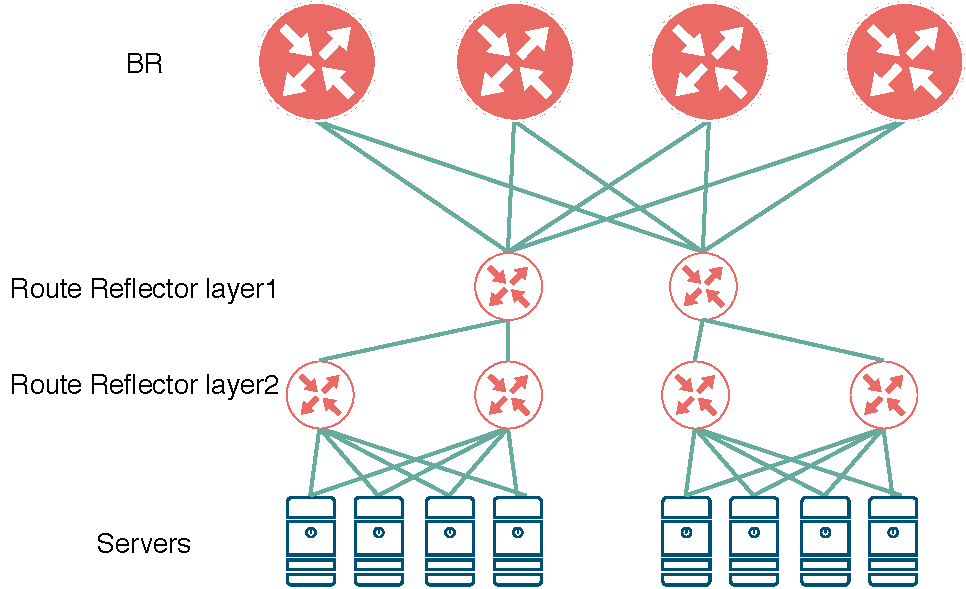
\includegraphics[width=12cm,pagebox=cropbox,clip]{img/2layer_bgp_topology_more_scale.pdf}
    \end{center}
    \caption{2層のBGPコネクショントポロジ}
    \label{fig:2layer_bgp_topology}
\end{figure}


また,本トポロジを採用したIDCネットワークにおける収容可能なサーバ数$S$は式\ref{eq:2layer_max_connection}のように示すことが出来る.この時,第一層のルートリフレクタの台数を2,BRのホスト数を$N$,第二層のルートリフレクタの台数を$L$,1台のルートリフレクタが収容可能なBGPピアの最大の数を$C_r$とする.


\begin{equation}
    S = \frac{L(C_r - N)}{2} \quad (L \leq C_r - N)
    \label{eq:2layer_max_connection}
\end{equation}


本研究において行った評価実験環境と同様に,1台のルートリフレクタが収容可能なBGPピア数$C_r$が630,BRの台数$N$が30である場合,本トポロジの最大収容可能サーバ数$S$は180000となる.

このようにBGPコネクショントポロジを多層化することで,BR及びIPv4サービス提供サーバが確立すべきコネクション数を増やすことなく,本提案手法のスケーラビリティをより高める事が可能になることがわかる.
同時に,本提案手法は数万台規模のサーバを抱える実際の商用ネットワークにおいても,本提案手法は高いスケーラビリティを有するモデルであると評価することが出来る.



% \subsection{EAMの集約}
% 本提案手法では,IPv4サービス提供サーバ自身がIPv4サービスアドレスを広告することを前提とした設計を行った.
% IPv4サービスアドレスを有するサーバ以外がEAMを複数集約して代理に広告するというユースケースを想定すると,BGPが利用するアドレスファミリの拡張仕様の設計が必要になると言える.


%%% Local Variables:
%%% mode: japanese-latex
%%% TeX-master: "../thesis"
%%% End:
